\subsection{s-t cuts in flow networks}

In graph, cuts are defined by dividing vertices into two parts and consist of the edges with one endpoint in each part. In flow networks s-t cuts are similar.

\begin{definition}
	An $s - t$ cut is defined by partitioning $V$ into $S$ and $T$, with $s \in S$, and $t \in T$.
\end{definition}

The difference between a cut in a graph and a cut in a flow network is as following: for a cut in a flow network, source $s$ and terminal $t$ must belongs to different sets.

\begin{definition}
	Forward edges are edges from set $S$ to set $T$. Backward edges are edges from set $T$ to set $S$.
\end{definition}
An example is as follows:
\begin{figure}[H]
	\centering
	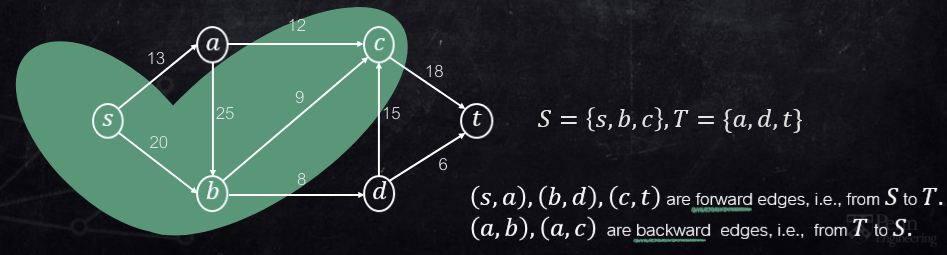
\includegraphics[width=0.8\textwidth]{fig/cut.png}
\end{figure}
\subsubsection{Notes}
For each cut $(S, T)$, any flow going from $s$ to $t$ must go from $S$ to $T$.

Because of conservation of flow, we can prove that $|f|$, the net flow out of $S$, is also the flow across any cut $(S, T)$ and the net flow into $t$.
\subsubsection{Example}
Imagine a city with a river running through it and only a few bridges across the river. The rate of traffic flow from the left bank to the right bank is limited by the rate that the bridges can bear.

Bridges form a cut. Removing them separates the left bank from the right; their capacity is a constraint on the amount of flow you can have.
\subsubsection{Capacity of a Cut}
The capacity of an $s-t$ cut $(S, T)$ should represent the maximum net flow you can send across the cut. Net flow across $(S, T)$ is sum of flows on forward edges minus sum of flows on backward edges. To send maximum net flow, must saturate the forward edges, and have 0 flow on the backward edges.
\begin{definition}
	The \textbf{capacity} of a cut is defined as the sum of the capacities of the forward edges of the cut.
\end{definition}

In the above example, the capacity of $s-t$ cut is $13 + 8 + 18 = 39$.

\subsubsection{Cut capacities and flow values}
Capacity of any $s-t$ cut is an \textbf{upper bound} on flow value of any flow. Cuts with small capacities are \textbf{bottlenecks}, like the bridges in a city. The minimum cut is the cut with the smallest capacity and the flow value must be no greater than this capacity.

\subsubsection{Correctness of Ford-Fulkerson}
\paragraph{Main idea:} If there are no paths from $s$ to $t$ in $G_f$, we know that Ford-Fulkerson terminates with flow $f$. So let us define a cut by letting $S$ be the set of all vertices reachable from $s$ in $G_f$. Let $T$ be the complementary set. We will show that the flow across this cut, and hence $|f|$ must be equal to the capacity of the cut, thereby proving that we have a max flow.

When Ford-Fulkerson terminates, we have an $s-t$ cut $(S-T)$ because $t$ is not
reachable from $s$ in $G_f$.

In the following example is a graph of net flow $G$, there are two kinds of edge $(u,v)$ and $(x,y)$. The former is from $S$ to $T$ and the latter is from $T$ to $S$. Recall one more time that $S$ and $T$ are chosen based on the residual graph $G_f$ but now we are looking at the original network graph $G$.

\begin{figure}[H]
	\centering
	
\includegraphics[width=0.5\textwidth]{fig/cut-2.png}
\end{figure}

Given such $S$ and $T$ sets, we can infer some nice properties for the forward edge and back edge.

\begin{itemize}
	\item Since, $u$ and $v$ are in different sets, there is no edge from $u$ to $v$ in $G_f$. It means $f(u, v)$ saturate its capacity in the network $G$.
	\item Since, $y$ and $x$ are in different sets, there is no edge from $y$ to $x$ in $G_f$. It means $f(x, y)$ must 0 in the network $G$ so that there is no residual in $G_f$.
\end{itemize}

So when Ford-Fulkerson stops, we have a cut (where $S$ contains vertices reachable from $S$) such that:
\begin{itemize}
	\item All forward edges are carrying as much flow as their capacity.
	\item All backward edges are carrying 0 flow.
\end{itemize}
Therefore, the flow across $(S, T)$ = cap$(S, T)$. Moreover, the flow across $(S, T) = |f|$.

Thus, the current flow is equal to the capacity of $(S, T)$ and then it must be optimal. Incidentally, we have found a min-cut, namely, $(S, T)$.

\subsection{Run Time Analysis}
Each iteration of the while loop:

\begin{itemize}
	\item Construct a residual graph: $O(m)$, where $m$ is the number of edges.
	\item Find a path from $s$ to $t$ in residual graph: $O(m)$ by dfs or bfs.
	\begin{itemize}
		\item Such a path is an augmenting path, because it augments the flow value.
	\end{itemize}
	\item Add the flow on this path to current flow: $O(m)$.
\end{itemize}

Number of iterations:
\begin{itemize}
	\item If all capacities are integers, each augmentation increases $|f|$ by at least 1.
	\item Maximum flow value is no more than the sum of capacities of edges leaving $s$.
	\item If we call this sum $C$, we have at most $C$ augmentations.
\end{itemize}

Total running time is $O(mC)$.










